% !TEX root = ThesisGchatzi.tex

\graphicspath{{Papers/SIGSpatial2017/}{Papers/SIGSpatial2018/}}

\section{Preliminaries}
\label{subsec:preliminaries}
Next, we introduce our notation and define the distance functions for geolocated time series.

In the {\em spatial domain}, the distance between two geolocated time series $T$ and $T'$ is calculated using the Euclidean distance of their respective locations. Furthermore, we normalize this distance with $maxDist_{sp}$, i.e., the maximum possible spatial distance in the dataset, to obtain a measure in the interval $[0,1]$. Thus:
\begin{equation} \label{eq:dist_sp}
 dist_{sp}(T, T') = \frac{\sqrt{(T.loc_x - T'.loc_x)^2 + (T.loc_y - T'.loc_y)^2}}{maxDist_{sp}}
\end{equation} \label{eq:2}

In the {\em time series domain}, similar to many prior works (e.g., \cite{shieh2008kdd}), we also apply the Euclidean distance to measure the similarity. Specifically, we calculate the distance between two geolocated time series $T$ and $T'$ as follows:
\begin{equation} \label{eq:dist_ts}
 dist_{ts}(T, T') = \frac{\sqrt{\displaystyle \sum_{i=1}^{w}(T.v_i - T'.v_i)^2}}{maxDist_{ts}}
\end{equation}

\noindent where $maxDist_{ts}$ denotes the maximum possible distance in the time series domain and is used for normalization, as above.

\section{The \tsr Index}
\label{subsec:tsr_tree}
This section presents the architecture of the \tsr index and its hybrid pruning capability both in the spatial and in the time series domain.

\subsection{Index Structure}
\label{subsec:index_structure}

The \tsr is an enhanced R-tree. As in the standard R-tree \cite{Guttman1984}, each node has at least $m$ and at most $M$ entries and stores the MBRs of its children. Additionally, for each child, a node stores a pair of \emph{Minimum Bounding Time Series} (MBTS) that enclose all the time series indexed in its subtree. More specifically, this pair consists of an \emph{upper bounding time series} $B^{\sqcap}$ and a \emph{lower bounding time series} $B^{\sqcup}$, respectively constructed by selecting the maximum (for $T^{\sqcap}$) and minimum (for $T^{\sqcup}$) of values at each time point among all geolocated time series indexed therein. More formally:

\begin{mydefinition} [Minimum Bounding Time Series (MBTS)]
Given a set of time series $\mathcal{T}$, its MBTS consists of an \emph{upper bounding time series} $B^{\sqcap}$ and a \emph{lower bounding time series} $B^{\sqcup}$, constructed by respectively selecting the maximum and minimum of values at each time point among all time series in set $\mathcal{T}$ as follows:
\begin{align}\label{eq:bounds}
 \begin{split}
  & B^{\sqcap} = \{ \max_{T \in \mathcal{T}} T.v_1, \ldots, \max_{T \in \mathcal{T}} T.v_{n} \} \\
  & B^{\sqcup} = \{ \min_{T \in \mathcal{T}} T.v_1, \ldots, \min_{T \in \mathcal{T}} T.v_{n} \}.
 \end{split}
\end{align}
\qed
\end{mydefinition}

\begin{figure}[!t]
 \centering
 \subfloat[MBTS in \tsr]{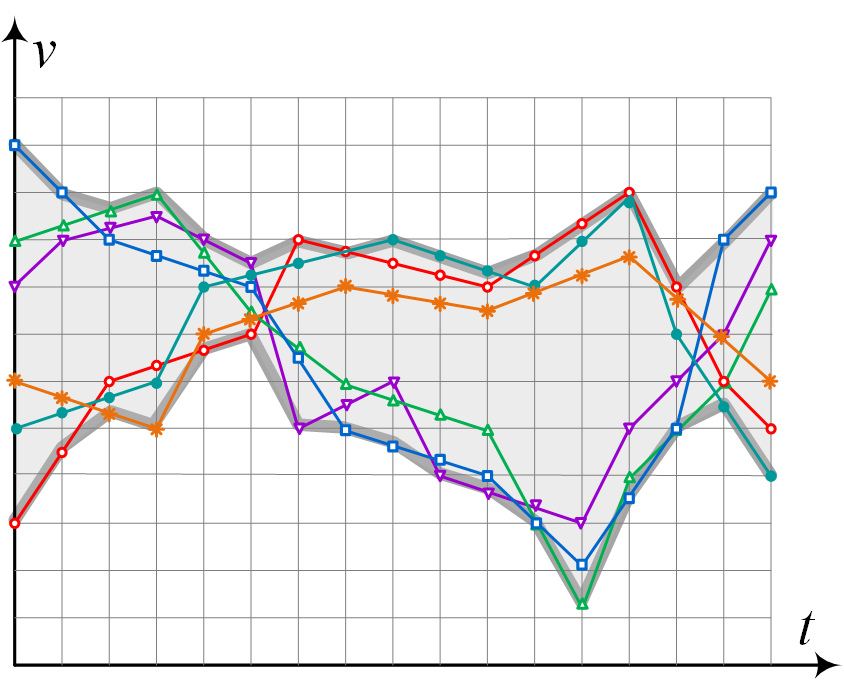
\includegraphics[width=0.3\textwidth]{figures/bounds_tsr.png}\label{subfig:tsr_mbts}}\hspace{8pt}
 \subfloat[Distance bounds with MBTS]{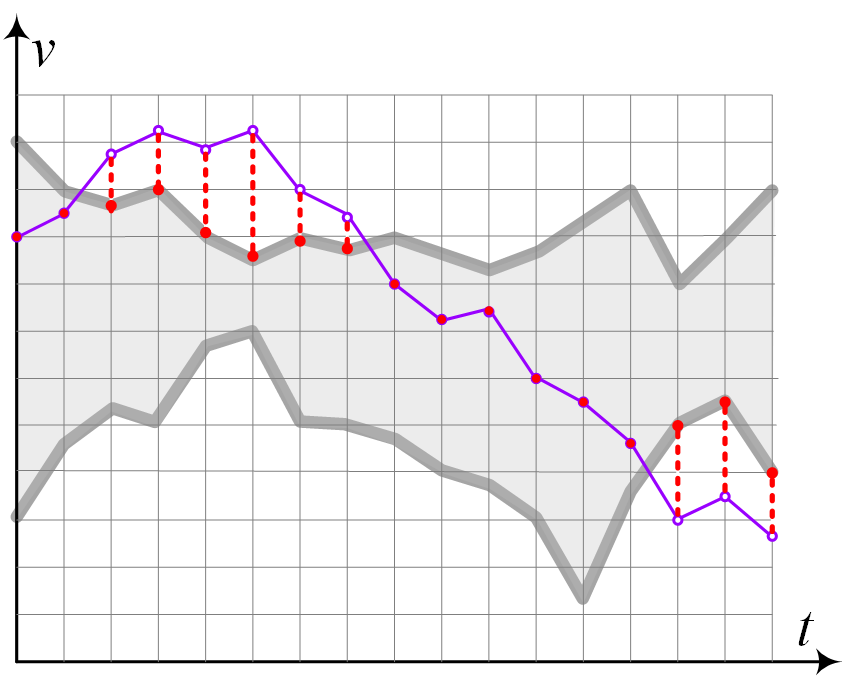
\includegraphics[width=0.3\textwidth]{figures/bounds_mindst.png}\label{subfig:mbts_bounds}}\hspace{8pt}
 \subfloat[MBTS in \btsr]{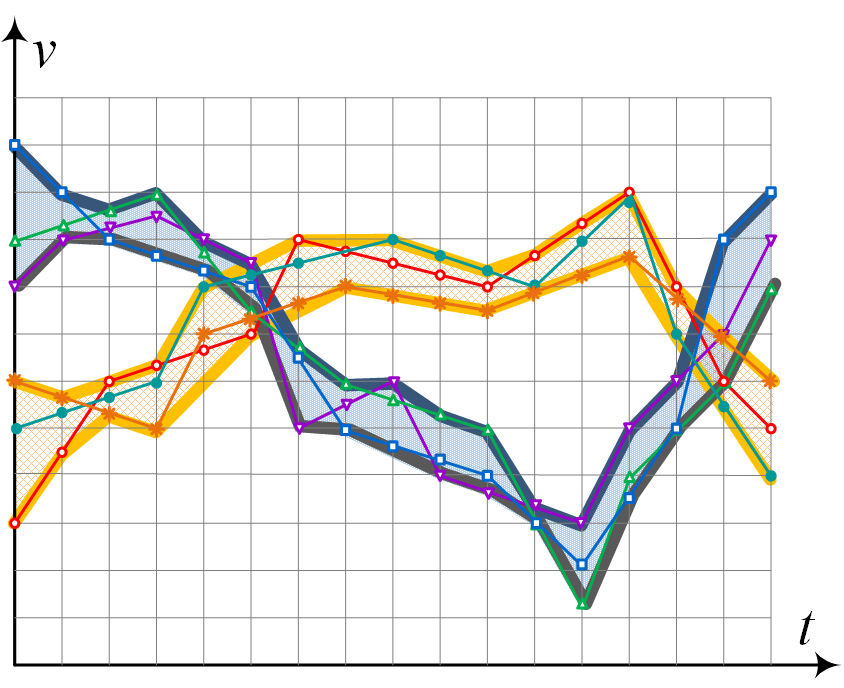
\includegraphics[width=0.3\textwidth]{figures/bounds_ctsr.png}\label{subfig:btsr_mbts}}
\caption{Examples illustrating the time series bounds and pruning in \tsr and \btsr.}
\label{fig:example_bounds}
\end{figure}

\begin{myexample}
 Figure \ref{subfig:tsr_mbts} illustrates an example of the MBTS of a set of given time series. The latter are represented in the figure by colored solid lines with different markers. The upper and lower bounding time series are represented by thick grey lines, enclosing the whole (shaded) area where the individual time series lie. \qed
\end{myexample}

Construction and maintenance of the \tsr follow the standard procedures of the R-tree for data insertion, deletion and node splitting. Raw geolocated time series are always inserted into leaves. The difference is that, after the R-tree has been built, it is traversed in a reverse breadth-first manner and the MBTS of each node are calculated. Moreover, the heuristic for determining where each geolocated time series will be inserted can be adapted to also account for the similarity in the time series domain, in addition to their spatial distance. Recall that in the standard R-tree, selecting the node where a new object will be inserted is based on finding the entry where such an insertion incurs the least possible enlargement of its MBR. Now, this is extended to also consider the enlargement incurred in that entry's MBTS. Specifically, selecting the appropriate node $N$ should minimize the following hybrid cost function:
\begin{equation}
 cost(T, N) = \lambda \cdot cost_{sp}(T, N) + (1 - \lambda) \cdot cost_{ts}(T, N)
 \label{eq:insertion_cost}
\end{equation}

\noindent where $T$ is the new geolocated time series for insertion, $cost_{sp}$ and $cost_{ts}$ are functions quantifying the cost of enlarging $N$'s MBR and MBTS, respectively, and $\lambda$ is a weight parameter determining the relative importance of the two factors. Notice that for $\lambda = 1$, this heuristic behaves exactly as in the standard R-tree. When checking a given geolocated time series $T$ for insertion in node $N$, we calculate distance $\delta_i$ between $T$ and current MBTS at each time point $i \in \{ 1, \dots, n \}$:
\begin{equation}
 \begin{split}
  \delta_i = \begin{cases}
	T.v_i - B^{\sqcap}_N.v_i, & \text{if} \;\; T.v_i > B^{\sqcap}_N.v_i \\
	B^{\sqcup}_N.v_i - T.v_i, & \text{if} \;\; T.v_i < B^{\sqcup}_N.v_i \\
	0, & \text{if} \;\; TB^{\sqcup}_N.v_i \leq T.v_i \leq B^{\sqcap}_N.v_i.
	  \end{cases}
 \end{split}
 \label{eq:delta_ts}
\end{equation}

\noindent Such distances $\delta_i$ are shown with dashed red lines in Figure~\ref{subfig:mbts_bounds}. Thus, we can quantify enlargement $cost_{ts} = \sum{\delta_i}$ of MBTS for $N$. 

\subsection{Hybrid Node Pruning}
\label{subsec:index_pruning}

For efficient hybrid query execution, the goal is to reduce the number of node accesses by pruning subtrees of the index that cannot contain any results. To do so, we need to establish lower bounds for the different types of distances between the query $T_q$ and any geolocated time series contained in the subtree rooted at a node $N$ in the index. In the spatial domain, this bounding $mindist_{sp}(T_q, N)$ is computed as in the case of the standard R-tree, i.e., based on $N's$ MBR. Similarly, in the time series domain, the corresponding bounding distance is derived by $N's$ MBTS. Following Equations \ref{eq:dist_ts} and \ref{eq:bounds}, it can be easily seen that this can be calculated as follows:

\begin{equation}
 mindist_{ts}(T_q, N) = \frac{\displaystyle \sqrt{\sum_{i=1}^{w} \delta_i^2}}{maxDist_{ts}}, \\
\label{eq:mindist_ts}
\end{equation}

\noindent where $\delta_i$ represents distances between $T_q$ and MBTS at each time point $i$, computed analogously to Equation~\ref{eq:delta_ts}.

\begin{myexample}
  Figure \ref{subfig:mbts_bounds} depicts a query time series (the magenta solid line) and the bounds (thick gray lines) in the MBTS of a node. The vertical dashed red lines outside MBTS indicate distances between the query and those bounds contributing to $mindist_{ts}(T_q, N_i)$. 
\end{myexample}

Moreover, given that the geolocated time series under a node $N$ are a subset of those of its parent $N'$, it follows from the definition of the time series bounds (Equation \ref{eq:bounds}) that the MBTS of $N$ is tighter than (or equal to) the MBTS of $N'$. From Equation \ref{eq:mindist_ts}, this guarantees that:

\begin{equation}
 mindist_{ts}(T_q, N') \leq mindist_{ts}(T_q, N).
\end{equation}

\noindent So, if $mindist_{ts}(T_q, N')$ is higher than threshold $\theta_{ts}$ specified by the query, the entire subtree rooted at $N'$ can be pruned altogether.

We define a {\em hybrid distance} measure $dist_h(T, T')$ between two geolocated time series $T$ and $T'$, combining both their distances $dist_{sp}(T, T')$ in the spatial domain and $dist_{ts}(T, T')$ in the time series domain. For that purpose, we apply an {\em exponential decay} function to decrease the similarity of two time series based on their spatial distance:
\begin{equation}
 sim_h(T, T') = sim_{ts}(T, T') \; e^{- \gamma \; dist_{sp}(T, T')}
 \label{eq:sim_h}
\end{equation}

\noindent where $sim_{ts}(T, T') = 1 - dist_{ts}(T, T')$ and $\gamma$ is the exponential decay constant. Then:
\begin{equation}
 dist_h(T, T') = 1 - sim_h(T, T')
 \label{eq:dist_h}
\end{equation}

Accordingly, the hybrid similarity (distance) between two geolocated time series $T$ and $T'$ is equal to their standard time series similarity (distance) if they are located at the same position, and it gradually decreases (respectively, increases) if one is placed farther apart from the other. From Equations \ref{eq:sim_h} and \ref{eq:dist_h} we can observe that hybrid distance $dist_h(T_q, T)$ is monotone with respect both to $dist_{sp}(T_q, T)$ and $dist_{ts}(T_q, T)$. This implies that a minimum hybrid distance bound $mindist_h(T_q, N)$ for the contents of a given node $N$ can be similarly established by combining the individual bounds $mindist_{sp}\\(T_q, N)$ and $mindist_{ts}(T_q, N)$, i.e.:

\begin{equation}
mindist_h(T_q, N) = 1 - (1 - mindist_{ts}(T_q, N)) \; e^{- \gamma \; mindist_{sp}(T_q, N)}
\end{equation}

\section{The BTSR-tree Index}
\label{sec:ctsrtree}

As explained in the previous section, each node in the \tsr holds an MBTS (i.e., a pair of upper and lower bounding time series) that encloses all the time series contained in its subtree. This allows to prune nodes while traversing the index by computing lower bounds for similarity in the time series domain. Clearly, the pruning effectiveness depends on the tightness of these bounds.

The \tsr does not provide any explicit guarantee that time series contained in the same node are highly similar to each other, hence the produced bounds are typically expected not to be sufficiently tight. Further, constructing the aggregate bounds from a set of dissimilar time series, yields bounding time series that are not very similar to any of the enclosed ones. These observations are obvious in the example of Figure \ref{subfig:tsr_mbts}, where the constructed MBTS encloses a much larger (grey shaded) area than the one actually occupied by the contained time series, and the resulting bounding time series do not closely resemble any of the original ones.

To overcome this issue, we present an optimized version of the \tsr, which we call \btsr. In a nutshell, the idea is to \emph{bundle} similar time series together in each node, and construct individual MBTS per bundle. This allows to derive bounding time series that are tighter and resemble more closely the enclosed ones. 

\begin{myexample}
 Figure \ref{subfig:btsr_mbts} illustrates this idea using the same example as Figure \ref{subfig:tsr_mbts}. The original time series are now grouped in two bundles, and the MBTS of each bundle is constructed separately. The resulting bounds are now much tighter, eliminating much of the dead space within the MBTS and allowing more precise similarity comparisons.
\end{myexample}

The \btsr index is built similarly to the \tsr index. To construct the time series bundles within each node, we rely on $k$-{\em means clustering}. To avoid confusion with the top-$k$ predicate in queries, next we symbolize with $\beta$ is the number of bundles to be created. The process is performed bottom-up, starting from the leaf nodes of the index. In each leaf node, the contained time series are clustered into $\beta$ bundles. Then, the MBTS of each bundle is computed and stored in the node. Each internal node receives all the MBTS of its children so as to compute its own $\beta$ bundles and respective set of MBTS. Thus, the process propagates upwards, until reaching the root of the tree.

\begin{figure}[!ht]
 \centering
 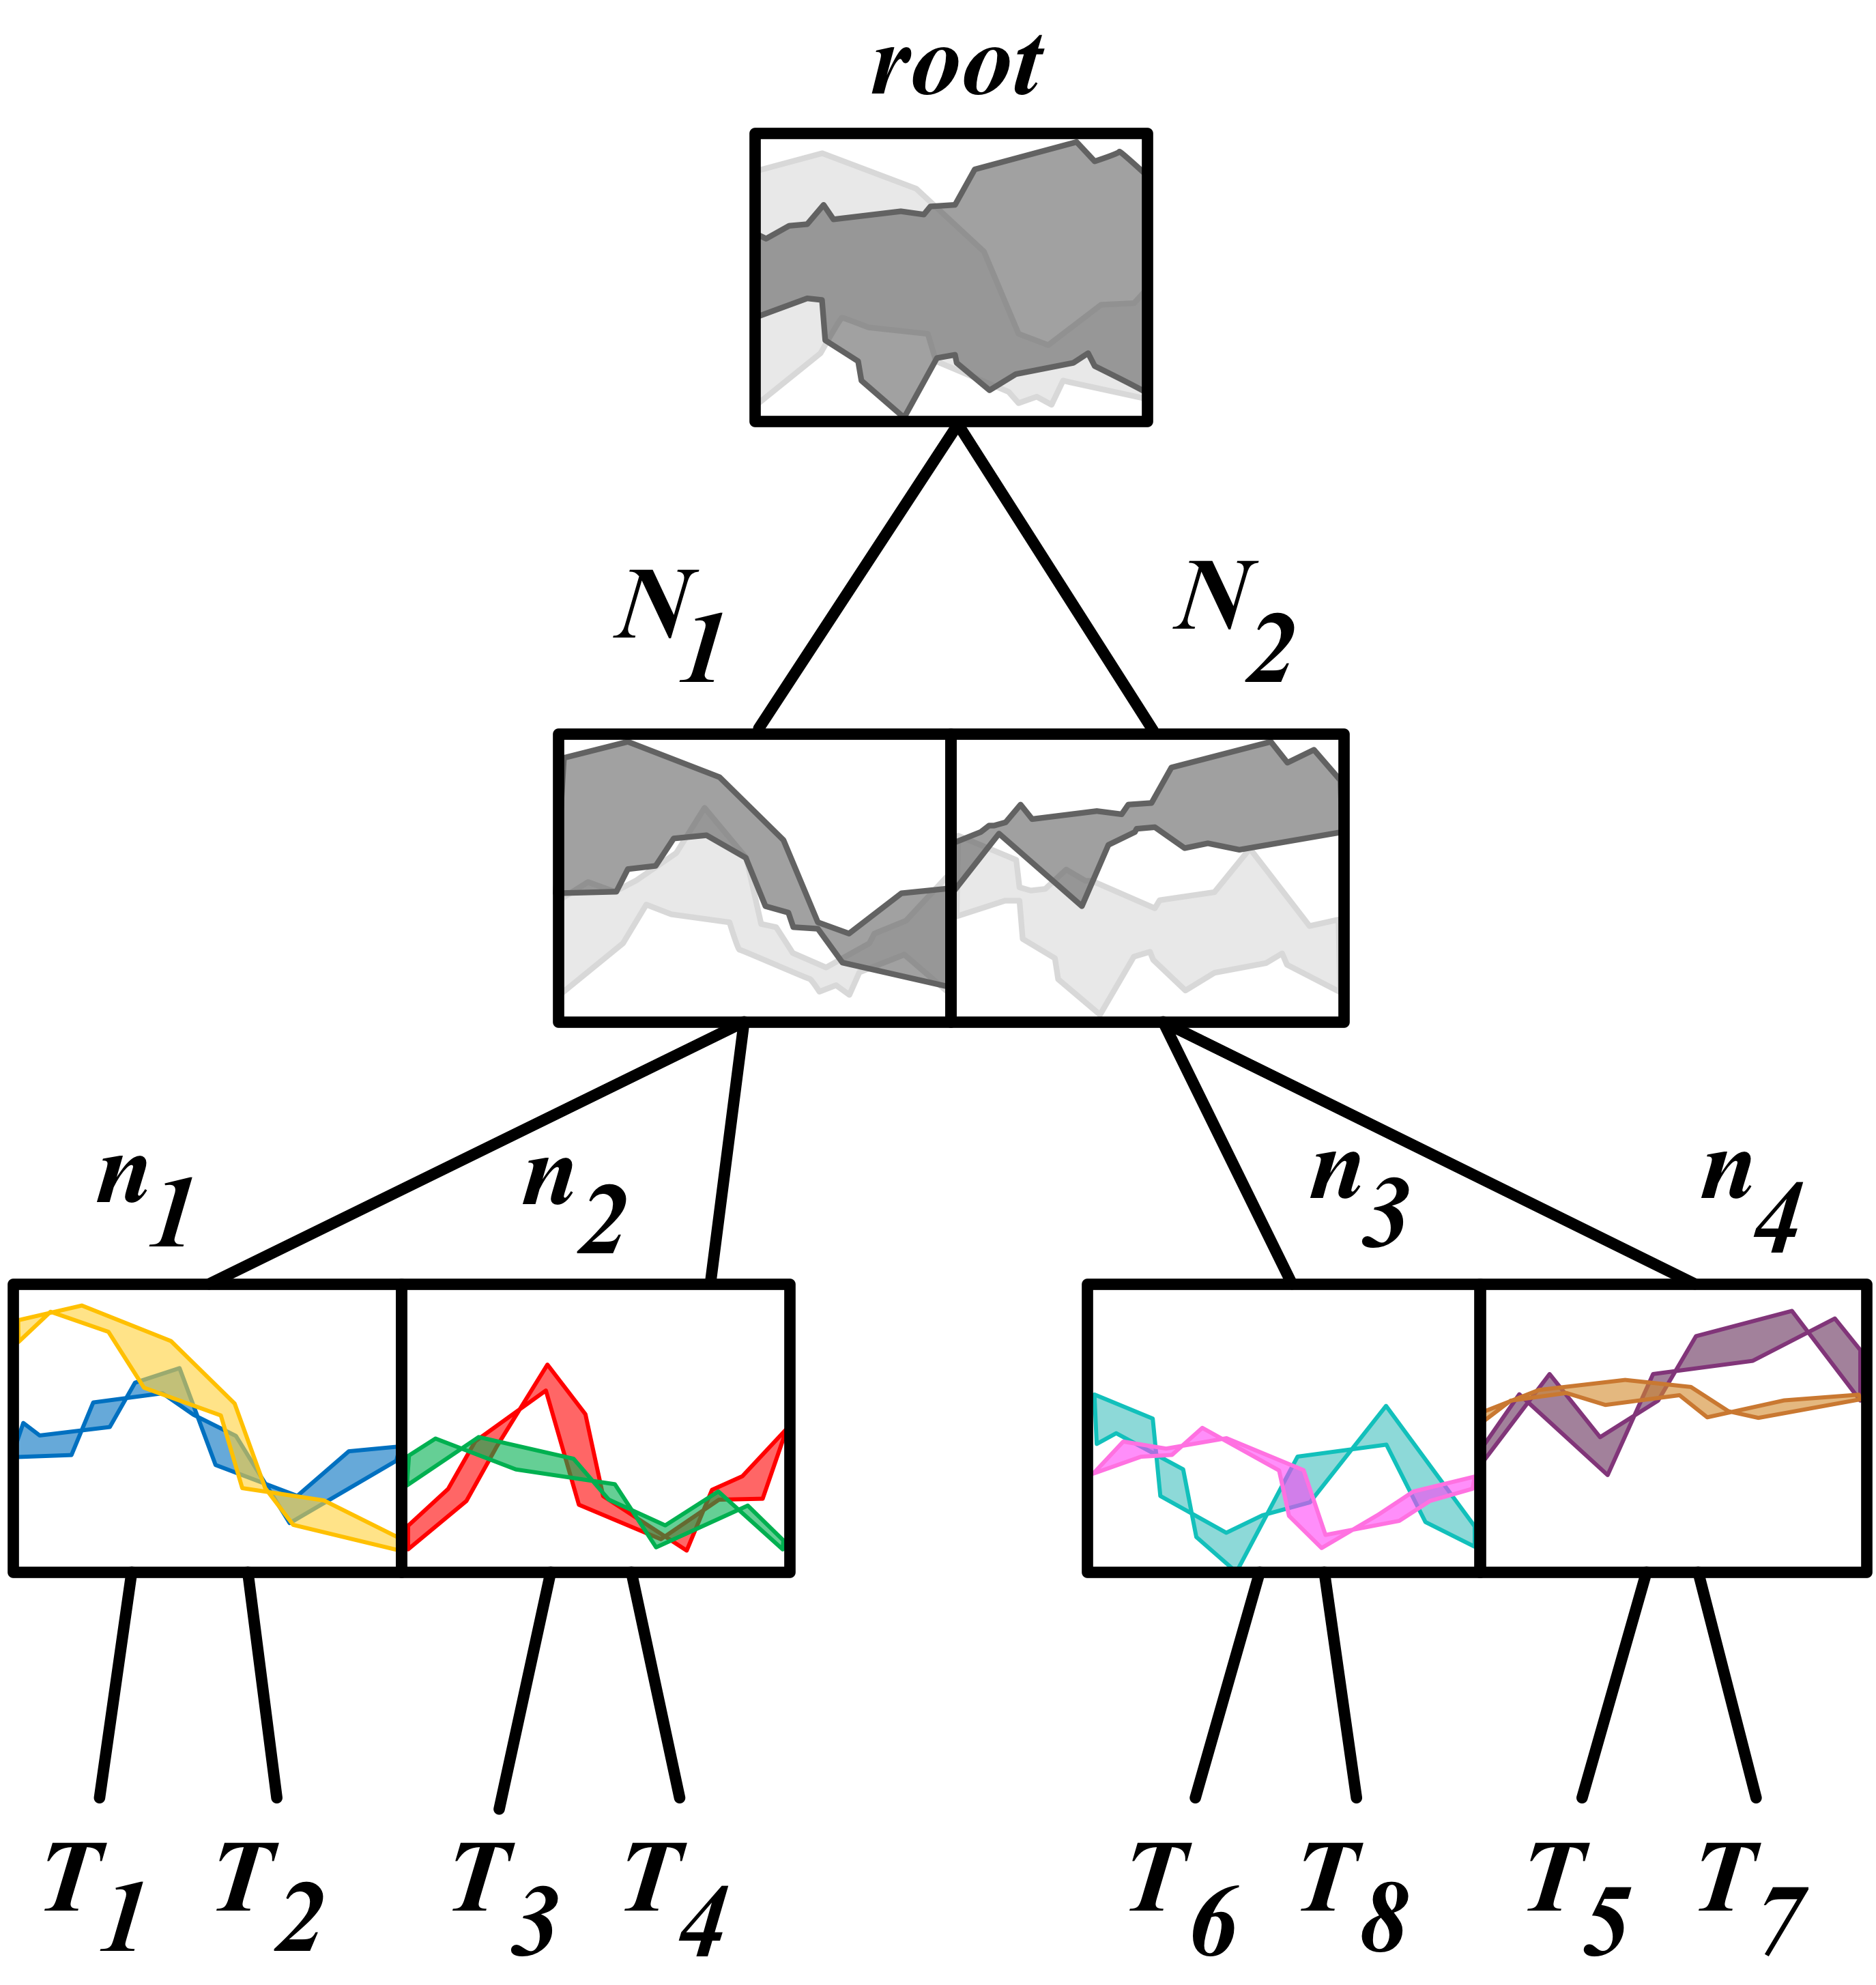
\includegraphics[width=0.75\textwidth]{figures/btsr_tree.png}
 \caption{An example of a \btsr index.}
 \label{fig:btsr_tree}
\end{figure}

Figure~\ref{fig:btsr_tree} depicts an example of a \btsr index for $\beta=2$. As described above, it is essentially a standard R-tree structure, with each node containing the necessary MBTS of its underlying geolocated time series. Notice that, as we move bottom-up towards the root of the tree, the MBTS of each node tend to be less and less tight and, consequently, overlap. Thus, a higher number $\beta$ of bundles is needed, since nodes become increasingly more heterogeneous in the time series they contain in their subtree. The higher the number $\beta$ of bundles, the tighter the resulting bounds. But this also implies that a larger number of MBTS needs to be maintained within each node. However, the number of bundles that can be created is limited by node capacity.

To address such issues, we increase the number of bundles bottom-up at every tree level by a factor $c$. Hence, a node at level $i$ has $\beta_{i} = c \cdot \beta_{i-1}$ bundles; at leaf level, such number $\beta_0$ is fixed. At the same time, in order to compensate this increase in terms of node capacity $M$, we decrease the resolution of the MBTS by the same factor $c$. The latter is achieved using PAA \cite{keogh2001paa,faloutsos2000vldb}. PAA is a common technique that can approximate a time series $T = \{v_1, \ldots, v_w\}$ of length $w$ into a time series $\bar{T} = \{\bar{v}_1, \ldots, \bar{v}_{w'}\}$ of any arbitrary length $w' \leq w$. In general, each $\bar{v}_i$ is calculated as follows:

\begin{equation}
 \bar{v}_i = \frac{w'}{w} \sum_{j = (w/w')(i-1)+1}^{(w/w')i} \; v_j
 \label{eq:paa_values}
\end{equation}

In our case, $w' = w / c$. To preserve bounds when applying PAA on an upper (lower) bounding time series $B^{\sqcap}$ ($B^{\sqcup}$), instead of taking the average as in Equation \ref{eq:paa_values}, we compute their max (min) values.

The \btsr can execute hybrid queries in a similar manner to the \tsr, with a straightforward adaptation. Whenever a node is accessed, instead of evaluating the pruning condition on a single pair of MBTS, each individual MBTS in each bundle is checked, and the node is pruned if all checks fail.